\section{Esqueleto funcional}
\label{sec:esqueleto}

El esqueleto prueba la única llamada directa entre servicios del sistema: Evaluación y actas le pregunta a Solicitudes y documentos por una solicitud, con gRPC, como decide el ADR-002. Son los dos servicios marcados con una estrella en el diagrama de contenedores (figura~\ref{fig:c4-n2}). El código está en la carpeta \nolinkurl{src/} del repositorio.

\subsection{Qué hace cada servicio}

\textbf{Solicitudes y documentos} (\nolinkurl{src/solicitudes/servidor.py}) es un servidor gRPC que escucha en el puerto 50051. Expone un solo método, \texttt{ConsultarSolicitud}, y responde siempre con los mismos datos: la solicitud está en estado \texttt{ENVIADA}, el informe y el reporte de URKUND están cargados y el porcentaje de coincidencia es 4,5~\%. Cada consulta que recibe la muestra en la consola con la hora.

\textbf{Evaluación y actas} (\nolinkurl{src/evaluacion/servicio.py}) es, por ahora, solo el cliente. Al arrancar consulta a Solicitudes por la solicitud \texttt{SOL-2026-001}, muestra la respuesta y termina. Espera la respuesta como máximo 5~segundos. Si Solicitudes no contesta, muestra el código de error de gRPC y termina sin seguir, que es lo que pide la sección~\ref{sec:cap-pacelc} para el porcentaje de URKUND.

Dejamos fuera la base de datos, el inicio de sesión, la rúbrica y las reglas del trámite, que llegan en E2. Los dos servicios están escritos en Python 3.13 con \texttt{grpcio} 1.85.3, el mismo entorno de PE-U1, porque ya sabíamos montarlo. El contrato no depende del lenguaje, así que sirve igual cuando los servicios pasen a Spring Boot.

\subsection{Contrato entre los dos servicios}

El código~\ref{lst:proto} es el contrato. Tiene un mensaje de consulta, con el identificador de la solicitud, y uno de respuesta, con los datos que Evaluación necesita antes de abrir la rúbrica. El código de Python se genera con \texttt{grpcio-tools} y se sube al repositorio, para que quien lo clone no tenga que generarlo.

\lstinputlisting[float=htbp,firstline=5,caption={Contrato gRPC del esqueleto (\texttt{src/proto/solicitudes.proto}).},label={lst:proto}]{../src/proto/solicitudes.proto}

\subsection{Cómo lo probamos}

La prueba sigue solo la sección ``Cómo ejecutar el esqueleto'' del README, en un clon limpio del repositorio:

\begin{enumerate}
  \item se clona el repositorio, se crea el entorno virtual y se instala \nolinkurl{requirements.txt};
  \item en una terminal se arranca Solicitudes con \texttt{python -m src.solicitudes.servidor};
  \item en otra terminal se ejecuta \texttt{python -m src.evaluacion.servicio}, y Evaluación muestra la respuesta mientras Solicitudes registra la consulta;
  \item se detiene Solicitudes y se ejecuta otra vez Evaluación, que debe mostrar \texttt{UNAVAILABLE} y terminar con código 1.
\end{enumerate}

Mario hizo la prueba primero en un clon limpio, antes de pasarla a Calidad: el 21 de noviembre de 2026 a las 21:55, en Windows 11. Los cuatro pasos de la lista se cumplieron, incluido el caso de Solicitudes apagado. Después, el 22 de noviembre de 2026, Jilmar clonó el repositorio en su máquina (DESKTOP-GTVSQ58) y siguió el README sin ayuda. Levantó Solicitudes en el puerto 50193 (figura~\ref{fig:captura-solicitudes}), y Evaluación recibió la respuesta y terminó con código~0 (figura~\ref{fig:captura-evaluacion}). Con Solicitudes detenido, Evaluación mostró \texttt{UNAVAILABLE} y terminó con código~1 (figura~\ref{fig:captura-apagado}). Las tres capturas se tomaron entre las 14:04 y las 14:05, muestran el usuario, el nombre de la máquina y la hora, y están en \nolinkurl{evidencias/capturas/}.

\begin{figure}[htbp]
  \centering
  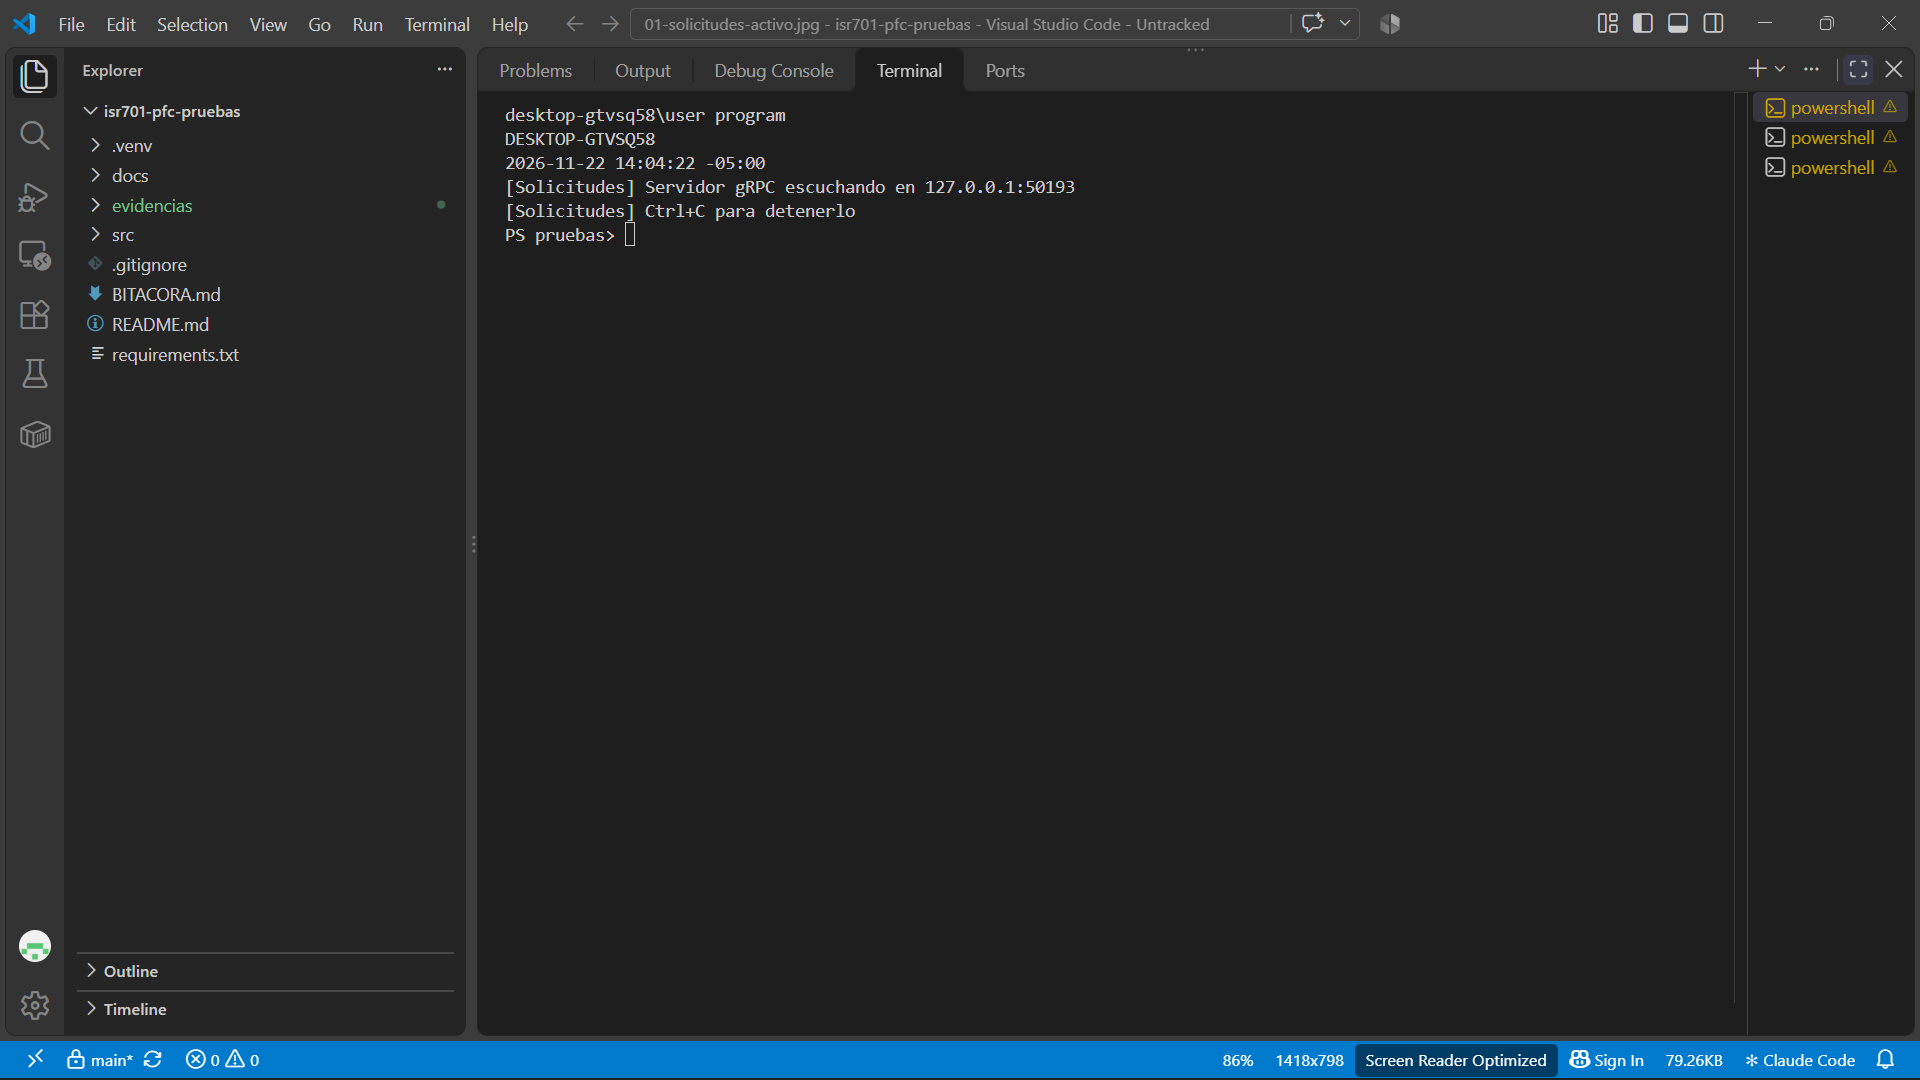
\includegraphics[width=\textwidth]{../evidencias/capturas/01-solicitudes-activo.png}
  \caption{Solicitudes escuchando en la máquina de Jilmar.}
  \label{fig:captura-solicitudes}
\end{figure}

\begin{figure}[htbp]
  \centering
  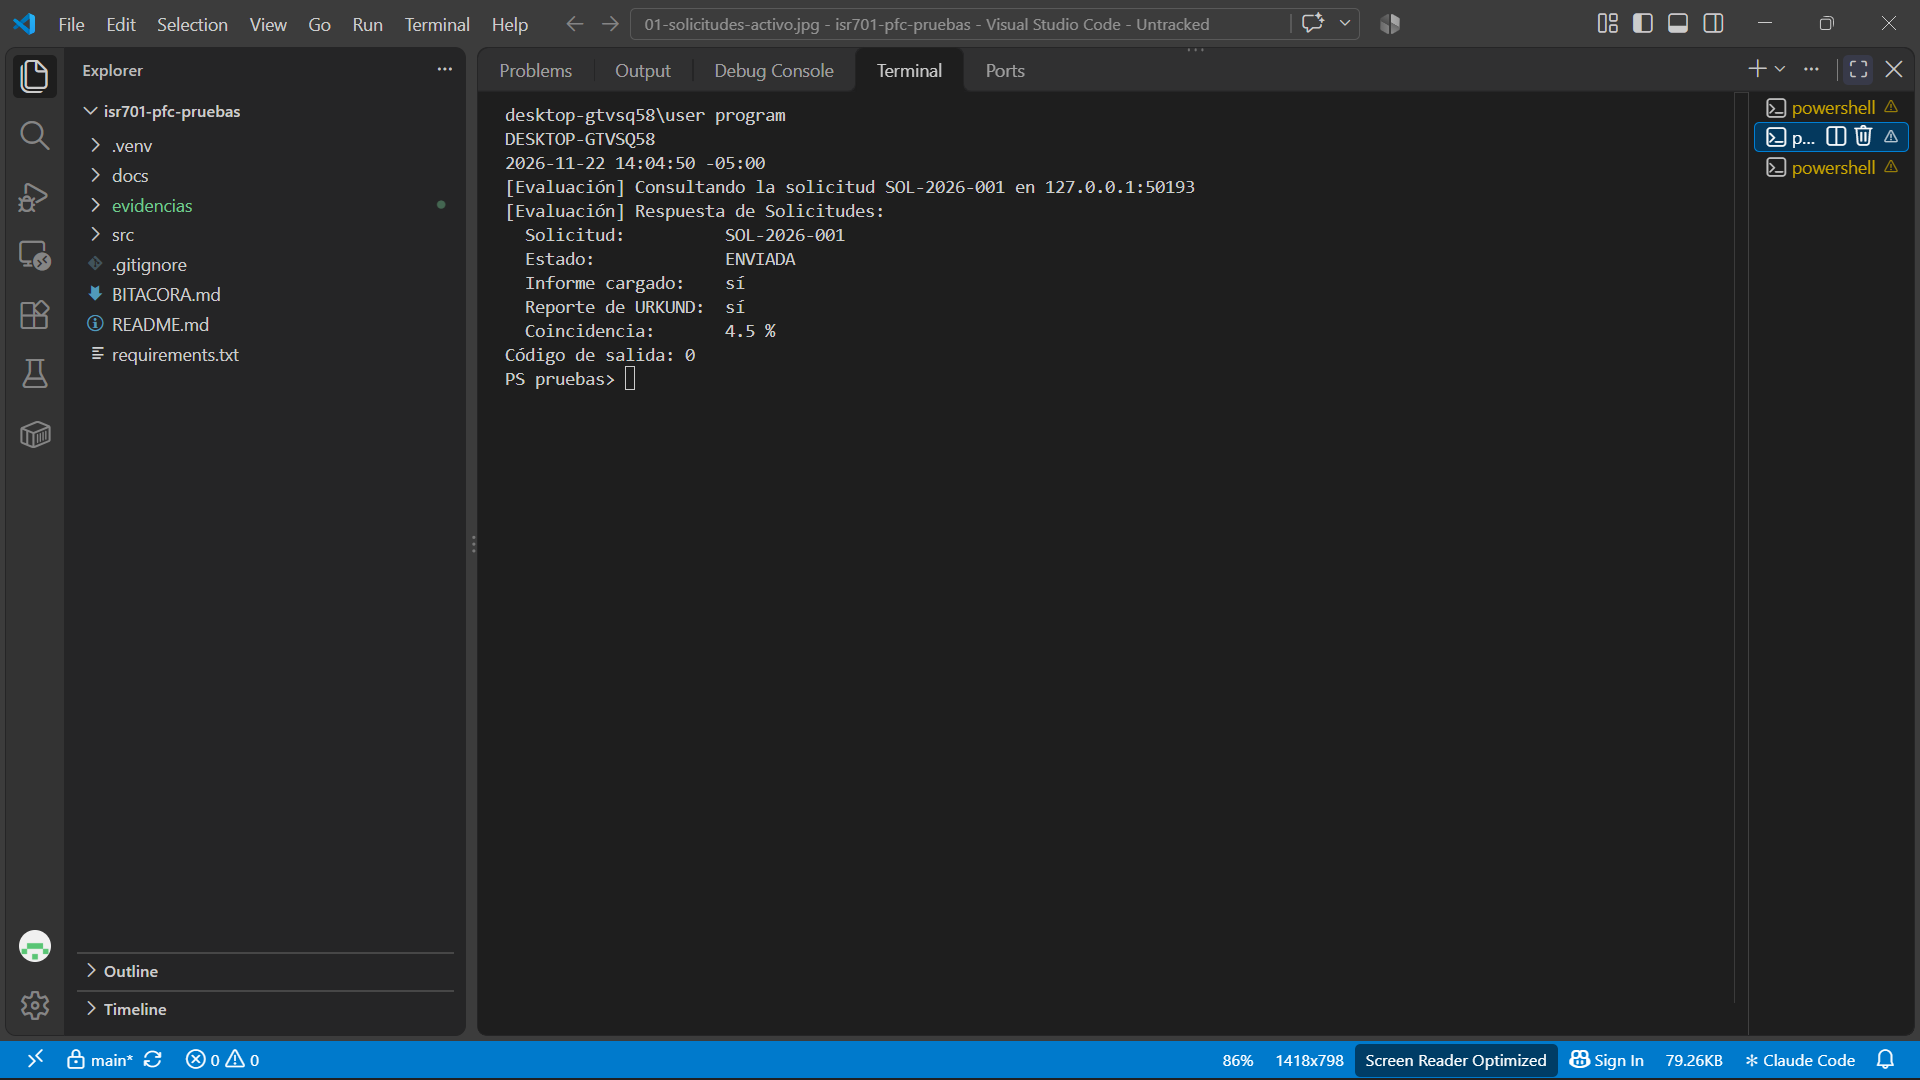
\includegraphics[width=\textwidth]{../evidencias/capturas/02-evaluacion-respuesta.png}
  \caption{Evaluación muestra la respuesta de Solicitudes y termina con código 0.}
  \label{fig:captura-evaluacion}
\end{figure}

\begin{figure}[htbp]
  \centering
  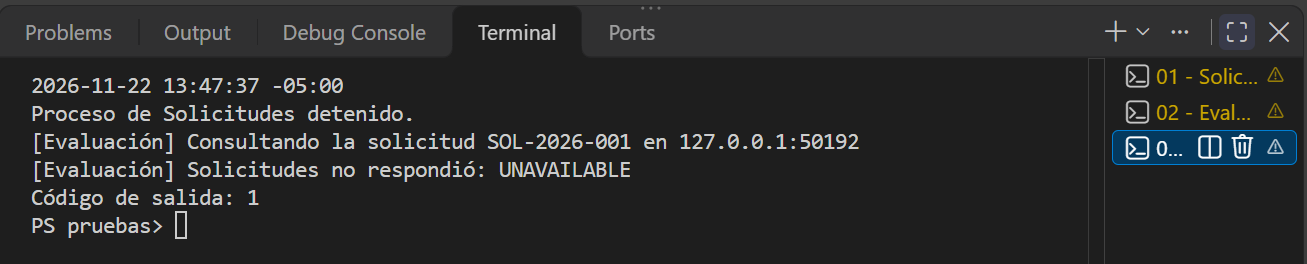
\includegraphics[width=\textwidth]{../evidencias/capturas/03-solicitudes-apagado.png}
  \caption{Con Solicitudes detenido, Evaluación muestra UNAVAILABLE y termina con código 1.}
  \label{fig:captura-apagado}
\end{figure}
